\documentclass[letterpaper, 12pt]{article}
\usepackage[letterpaper, top=2.5cm, bottom=2.5cm, left=3cm, right=3cm]{geometry} %margenes
\usepackage[utf8]{inputenc} %manejo de caracteres especiales
\usepackage[spanish]{babel} %manejo de encabezados de inglés a español
\usepackage{fancyhdr} %formato de los encabezados de página
\usepackage{ragged2e} %alineado real justficado
\usepackage{graphicx} %manejo de imagenes
\usepackage{amsmath} %manejo de notación matemática
\usepackage{mathtools} %manejo de notación matemática
\usepackage{blindtext} %texto de relleno
\usepackage{cancel} %permite la simbolización de cancelación de terminos
\usepackage{enumitem}[shortlabels] %listas con letras
\usepackage{amssymb} %manejo de simbolog►1a matematica

\pagestyle{fancy}
\fancyhf{}
\rfoot{\thepage}

\begin{document}

\setcounter{page}{1}
\thispagestyle{fancy}
\lhead{\textbf{Tarea 5, U1}}
\rhead{\textbf{23/09/2020}}
\section{Vectores en el espacio}
\subsection*{Dados \(\vec{u}=<\!4,1\!>\) y \(\vec{v}=<\!2,3\!>\) obtener \(\text{proy}_{\vec{v}}\vec{u}\) y \(\text{proy}_{\vec{u}}\vec{v}\) }
\subsection*{Gráfica:}
\centering
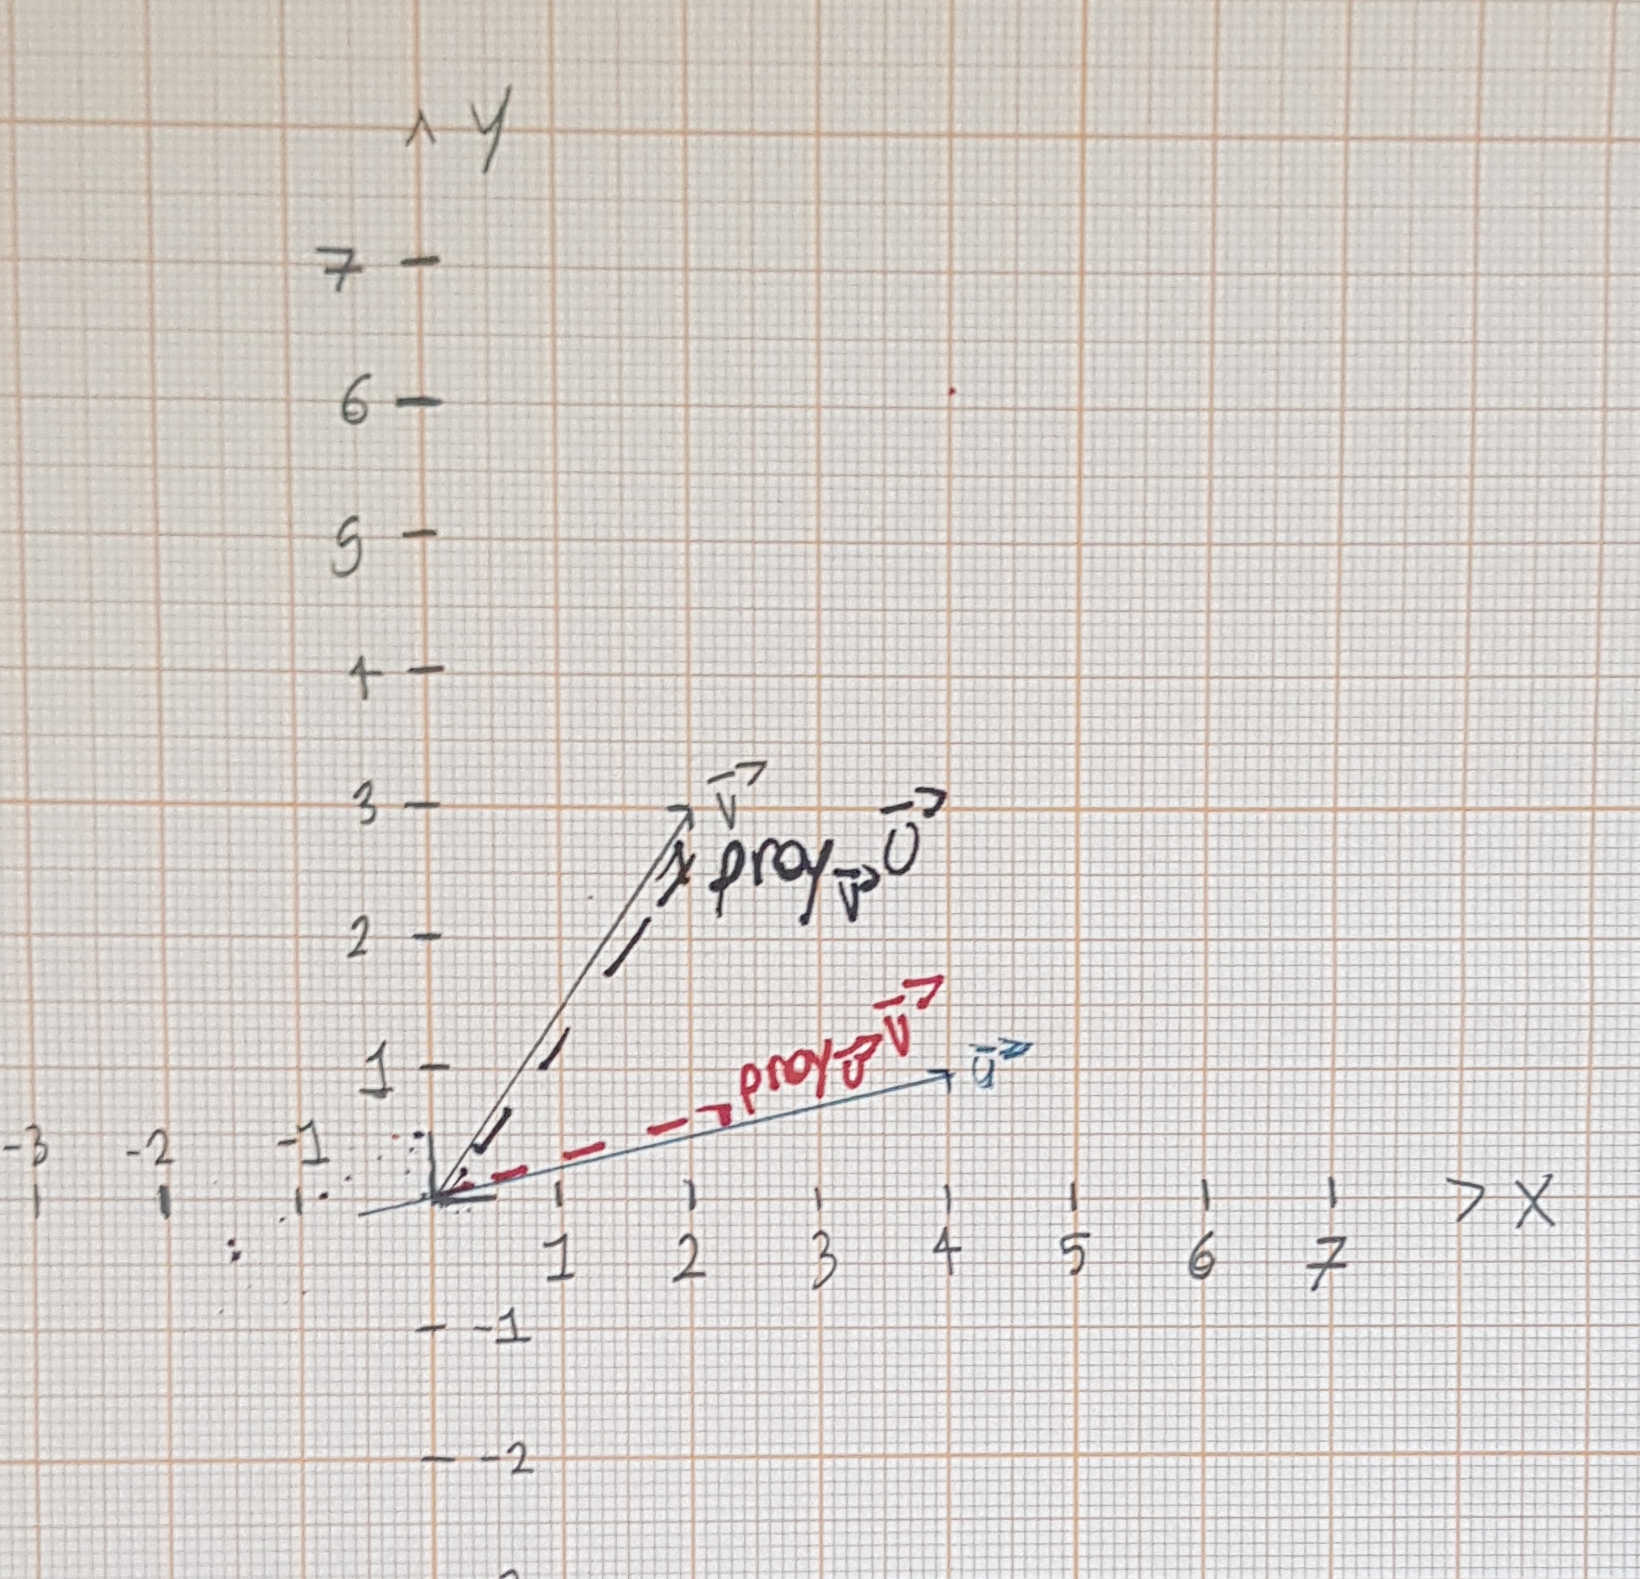
\includegraphics[width=13cm]{grafica.jpg}
\justify
\subsection*{Cálculos:}
\justify
Como se habló en clase, debemos usar las sig. fórmulas:
\[\text{comp}_{\vec{v}}\vec{u}=\lVert\vec{u}\rVert\cos\theta\left(\lambda\vec{v}\right)=\frac{\vec{u}\cdot\vec{v}}{\lVert\vec{v}\rVert}\leftarrow\text{escalar}\]
\[\text{proy}_{\vec{v}}\vec{u}=\text{comp}_{\vec{v}}\vec{u}\left(\lambda\vec{v}\right)=\frac{\vec{u}\cdot\vec{v}}{\lVert\vec{v}\rVert^2}\cdot\vec{v}\leftarrow\text{vector}\]
\textbf{\(\text{proy}_{\vec{v}}\vec{u}\):}\\ \newline
\(\text{comp}_{\vec{v}}\vec{u}=\frac{\vec{u}\cdot\vec{v}}{\lVert\vec{v}\rVert};\,\vec{u}\cdot\vec{v}=u_1v_1+u_2v_2=4(2)+1(3)=8+3=11;\)\\
\(\lVert\vec{v}\rVert=\sqrt{v_1^2+v_2^2}=\sqrt{2^2+3^2}=\sqrt{4+9}=\sqrt{13}\therefore \text{comp}_{\vec{v}}\vec{u}=\frac{11}{\sqrt{13}}\therefore \text{proy}_{\vec{v}}\vec{u}=\)\\
\(\text{comp}_{\vec{v}}\vec{u}\left(\lambda \vec{v}\right)=\left(\frac{11}{\sqrt{13}}\right)\!<\!\frac{2}{\sqrt{13}},\frac{3}{\sqrt{13}}\!>=<\!\frac{22}{13},\frac{33}{13}\!>\)\\
\textbf{\(\text{proy}_{\vec{u}}\vec{v}\):}\\ \newline
\(\text{comp}_{\vec{u}}\vec{v}=\frac{\vec{u}\cdot\vec{v}}{\lVert\vec{u}\rVert};\,\lVert\vec{u}\rVert=\sqrt{u_1^2+u_2^2}=\sqrt{4^2+1^2}=\sqrt{16+1}=\sqrt{17}\therefore\text{comp}_{\vec{v}}\vec{u}=\frac{11}{\sqrt{17}}\therefore\)\\
\(\text{proy}_{\vec{u}}\vec{v}=\text{comp}_{\vec{u}}\vec{v}\left(\lambda \vec{u}\right)=\left(\frac{11}{\sqrt{17}}\right)\!<\!\frac{4}{\sqrt{17}},\frac{1}{\sqrt{17}}\!>=<\!\frac{44}{17},\frac{11}{17}\!>\)\\ \newline
Dando por concluido la cuestión.
\end{document}